% Original course schematic of a degree-K state approximation on one finite
% element. The mathematical layout follows Biegler (2010), Fig. 10.1, but this
% is a fresh vector drawing rather than a reproduction of the textbook image.

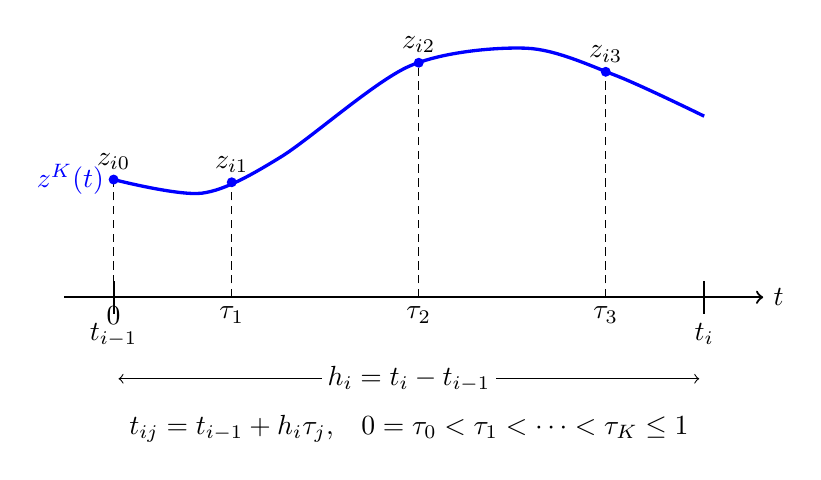
\begin{tikzpicture}[x=1.25cm,y=1.15cm]
  % Normalized-time axis and element endpoints.
  \draw[->,thick] (0,0) -- (7.1,0) node[right] {$t$};
  \draw[thick] (0.5,-0.18) -- (0.5,0.18);
  \draw[thick] (6.5,-0.18) -- (6.5,0.18);
  \node[below] at (0.5,-0.18) {$t_{i-1}$};
  \node[below] at (6.5,-0.18) {$t_i$};
  \draw[<->] (0.55,-0.9) -- (6.45,-0.9)
    node[midway,fill=white,inner sep=2pt] {$h_i=t_i-t_{i-1}$};

  % A generic polynomial state profile and its interpolation values.
  \draw[blue,very thick]
    plot[smooth] coordinates {(0.5,1.3) (1.4,1.15) (2.2,1.55)
      (3.5,2.55) (4.7,2.75) (5.6,2.45) (6.5,2.0)};
  \node[left,blue] at (0.5,1.3) {$z^K(t)$};

  \foreach \x/\taulabel/\lab/\y in {
      0.5/0/z_{i0}/1.3,
      1.7/\tau_1/z_{i1}/1.27,
      3.6/\tau_2/z_{i2}/2.59,
      5.5/\tau_3/z_{i3}/2.49} {
    \draw[densely dashed] (\x,0) -- (\x,\y);
    \fill[blue] (\x,\y) circle (1.8pt);
    \node[above] at (\x,\y) {$\lab$};
    \node[below] at (\x,0) {$\taulabel$};
  }

  \node[align=center] at (3.5,-1.45)
    {$t_{ij}=t_{i-1}+h_i\tau_j$,\quad $0=\tau_0<\tau_1<\cdots<\tau_K\leq 1$};
\end{tikzpicture}
